\documentclass{standalone}
\usepackage{tikz}
\usepackage{ctex,siunitx}
\usepackage{tkz-euclide}
\usepackage{amsmath}
\usetikzlibrary{patterns, calc}
\usetikzlibrary {decorations.pathmorphing, decorations.pathreplacing, decorations.shapes,}
\begin{document}
\small
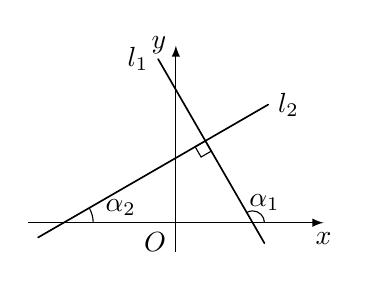
\begin{tikzpicture}[>=latex,scale=0.75]
  \begin{scope}
    \draw[thin,->](-2.5,0)--(2.5,0)node[below]{$x$};
    \draw[thin,->](0,-0.5)--(0,3.0)node[left]{$y$};
    \tkzDefPoints{1.3/0/A,-1.9/0/B,3/0/E,0/0/O}
    \tkzDefShiftPoint[B](30:2.0){C}
    \tkzDefPointBy[projection=onto B--C](A)\tkzGetPoint{D}
    \tkzDrawLine[semithick,add = 0.25 and 1.0](B,C)
    \tkzLabelLine[pos=2.0,right](B,C){$l_2$}
    \tkzDrawLine[semithick,add = 0.25 and 1.0](A,D)
    \tkzLabelLine[pos=2.0,left](A,D){$l_1$}
    \tkzMarkAngle[size=0.5](A,B,D)
    \tkzLabelAngle[pos=1.0](A,B,D){$\alpha_2$}
    \tkzMarkAngle[size=0.2](E,A,D)
    \tkzLabelAngle[pos=0.4](E,A,D){$\alpha_1$}
    \tkzMarkRightAngle[size=0.2](A,D,B)
    \tkzLabelPoints[below left](O)
  \end{scope}
\end{tikzpicture}
\end{document}